\documentclass[tikz]{standalone}
\usepackage{amsmath}
\begin{document}
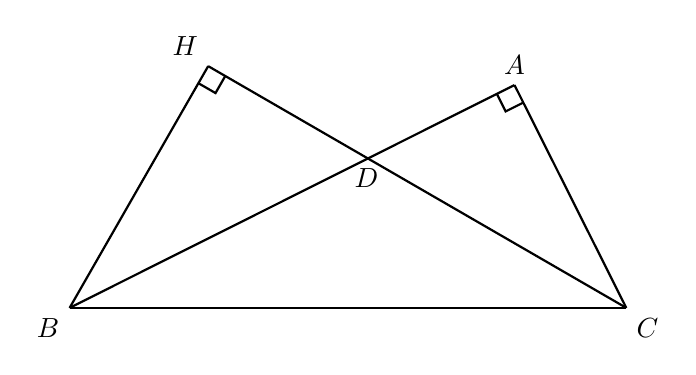
\begin{tikzpicture}[line width=0.8pt]
  % 顶点坐标
  \coordinate (B) at (0,0);
  \coordinate (C) at (7.07,0);
  \coordinate (A) at (5.65,2.83);
  \coordinate (H) at (1.76,3.07);
  \coordinate (D) at (3.77,1.90);

  % 线段
  \draw (B) -- (C);
  \draw (B) -- (H);
  \draw (H) -- (C);
  \draw (B) -- (A);
  \draw (A) -- (C);

  % 直角标记（在 H 处）
  \draw (1.636,2.853) -- (1.853,2.728) -- (1.977,2.945);
  % 直角标记（在 A 处）
  \draw (5.426,2.718) -- (5.538,2.495) -- (5.762,2.607);

  % 标签
  \node[above left] at (H) {$H$};
  \node[above] at (A) {$A$};
  \node[below] at (D) {$D$};
  \node[below left] at (B) {$B$};
  \node[below right] at (C) {$C$};
\end{tikzpicture}
\end{document}
